Despite being two different devices, the smartphone and Google Glass, Google's design recommendations share similarities. For instance, similar to Google's design guidelines for Google Glass Google recommend developers to keep information brief. Google recommend developers to use short phrases with simple words~\cite{androidDesignPrinciples}.

However, in contrast to Google's design guidelines for Google Glass, Google does give developers freedom to make their own decisions. ``Deviate with purpose'', as Google states. Google recommend developers to develop applications which are easy and fun to use. Google also recommend the use of pictures and icons rather than menus and buttons.

Most of all Google encourage developers to simply help users, but to ultimately let users decide for themselves. Applications designed for smartphones should make users feel as if they are skilled and in control, as well as remember what the user has done previously.

An example of how developers might make users feel powerful is for instance by, in a image editor application, give users tools which applies multiple effects at the same time. In terms of remembering what the user did previously an example is to remember what the user has entered in a text field previously, and displaying previous results in a drop-down menu as the user starts typing in the text same field the next time, as seen in Figure~\ref{smartphonePrinciples1}

	\begin{figure}[ht!]
		\centering
		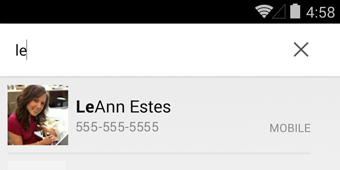
\includegraphics[width=110mm]{images/principles_get_to_know_me}
		\caption{Remember what the user has done previously~\cite{androidDesignPrinciples}.}
		\label{smartphonePrinciples1}
	\end{figure}

Another design guideline for applications on smartphones provided by Google is to highlight what is most important in the application. For instance, in a camera application what is most important is the shutter button. As such the shutter button should be the most prominent component in the application and easy to find, similar to Figure~\ref{smartphonePrincinples2}, making the application easy to use in terms of the core feature.

	\begin{figure}[ht!]
		\centering
		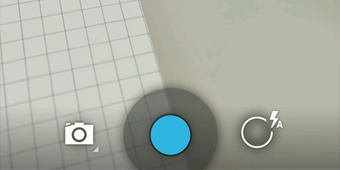
\includegraphics[width=110mm]{images/principles_make_important_fast}
		\caption{The most important component should be the most prominent~\cite{androidDesignPrinciples}.}
		\label{smartphonePrincinples2}
	\end{figure}

% Google ask developers who are designing for smartphones to think of simplicity and clarity. Google put much emphasis on making applications easy to use.

%However, there are some differences. For smartphones Google also recommend developers to keep track of what users have done in the past. Google ask developers to remember the user's input history and customisation in order to make the experience more pleasant for returning users~\cite{androidDesignPrinciples}.

%Google differ in how they want developers to design applications for smartphones and Google Glass respectively. On smartphones, Google are much more open to developers using their own ideas. Google encourage freedom and give more subtle hints of how to design in contrast to the more strict guidelines for Google Glass. For instance, Google want developers to make applications for smartphones fun and easy to use. They recommend consistency and a rewarding application.

In terms of clear cut differences between designing applications for smartphones compared to designing applications for Google Glass the most important one is perhaps where the user touches on the device. The Google Glass touchpad is mounted on the right hand side of the user, while the display sits in front of the user. On a smartphone the display and the touch-area is the same area. As such, buttons and other similar, intuitive, touch-objects are well suited for applications on smartphones. On Google Glass the user does not have any pointer on the screen, meaning that, for instance, menus can not be dependent on the user selecting an option by touching the option on the screen.

The use of voice command on Google Glass does help menus on Google Glass seem more similar to those on a smartphone since the users may select an option with their voice. However, the use of buttons and icons is less practical. On the other hand, since Google Glass may be controlled by voice command, developers might also hide functionality and decide not to show buttons and icons on the screen since the user does not need a target to touch in order to interact with the application.

An example of where Google Glass might hide functionality is in a camera application. In Figure~\ref{smartphonePrincinples2} part of a camera application for smartphones is shown, with three buttons on screen. An application for Google Glass would not need to display any buttons since the users need only to say what they want to do. If, however, the Google Glass user did not use the voice command functionality, a simple touch of the Google Glass touchpad might for instance bring up a menu, displaying possible options, similar to how saying ``ok glass'' would bring up the voice menu.

All the above guidelines and restrictions have been taken in to consideration when designing the application for smartphone as well as Google Glass. While the application does have the same functionality, the most noticable difference between the two applications is that the smartphone application have buttons, enabling the user to jump forward, past slides to reach, for instance, the instructions, where as in the Google Glass application such features have been limited to voice commands.